\documentclass[12pt]{article}
\usepackage[utf8]{inputenc}

\usepackage[letterpaper,margin=1in]{geometry}

\usepackage[style=apa,sorting=nyt]{biblatex}
\addbibresource{abstract.bib}

%\usepackage{graphicx}
%\graphicspath{{./images/}}

\usepackage[compact]{titlesec}
% \titleformat{\section}[runin]{\normalfont\large\bfseries}{}{0em}{}

\usepackage{hyperref}

% Formerly
% \title{\vspace{-5ex} \textbf{How fast did Cicero speak?} \\ \normalsize The speech rate of Classical Latin versus its Romance descendants \vspace{-5ex}}
% (with no author)
\title{\vspace{-5ex} \Large \textbf{How fast did Cicero speak?} \\ \large The speech rate of Classical Latin versus its Romance descendants \vspace{-3.5ex}}
\author{\normalsize Daniel Stelzer, University of Illinois at Urbana-Champaign}
\date{\vspace{-5ex}}

\usepackage{tipa}

\begin{document}

\maketitle

\section{Overview}

% Intro?

In 2019, Coupé et al demonstrated experimentally that, while rate of speech (syllables spoken per second) and information density (bits conveyed per syllable) vary significantly between languages, their product (bits conveyed per second) does not. This ``information rate'' seems to be a property of the communicative niche of human language in general, a true linguistic universal.

Coupé approximated information density as the \emph{syllable-conditional entropy}: the average amount of information conveyed by a single syllable, given knowledge of what syllable came before it. And while his method of measuring speech rate is impossible without living native speakers, the syllable-conditional entropy can be calculated from a purely written corpus (after Oh (2015)), by measuring the frequencies of all syllables and contexts.

In their previous studies, Coupé and Oh mostly used corpora with tens or hundreds of millions of tokens. However, most corpora for dead languages are significantly smaller than this; the entire surviving body of Classical Latin literature, for example, has barely over two million, on an order of magnitude with just two weeks of the \emph{New York Times}.

To compensate for this, we developed new methods to extrapolate from a limited corpus, showing what the entropy would be if the corpus were infinitely large, and how much uncertainty results from the limited sample size. Using these new methods on the Packard Humanities Institute corpus, we were able to estimate the information density for Classical Latin. From this we can predict the natural rate of speech of the Romans during the classical era, and compare it to that of modern Romance languages.

\section{Methods}

The first step in calculating information density involved converting the Latin text to a phonemic representation, generally following Allen (1978). The phonemic form is almost entirely predictable from the written form, with only a few exceptions: standard Latin orthography doesn't indicate vowel length or distinguish vowels from approximants.

These exceptions were handled automatically using a system developed by Winge (2015), which has been shown to disambiguate Latin orthography with over 98\% accuracy. The rest of the preprocessing involved giving every phoneme an unambiguous representation and calculating syllable breaks, using a modified version of an algorithm by Johnson (2019). The only non-phonemic detail included was neutralization: if the distinction between two phonemes was completely lost in a particular environment, that distinction was removed in preprocessing.

Next, we had to compensate for the size of the corpus. As Oh noted, as the corpus size increases, the estimated entropy grows sharply at first, then levels off and converges. By artificially reducing larger corpora (discarding a certain number of tokens at random), we determined experimentally that this growth follows a negative power function \( H = a_1 - a_2 (x - a_3)^{-a_4} \); fitting this function to the data with least squares then shows what value the entropy would converge to if our corpus were infinitely large.

%\begin{figure}[h]
%\caption{Estimated entropy of English (red) and Latin (blue), as a function of corpus size}
%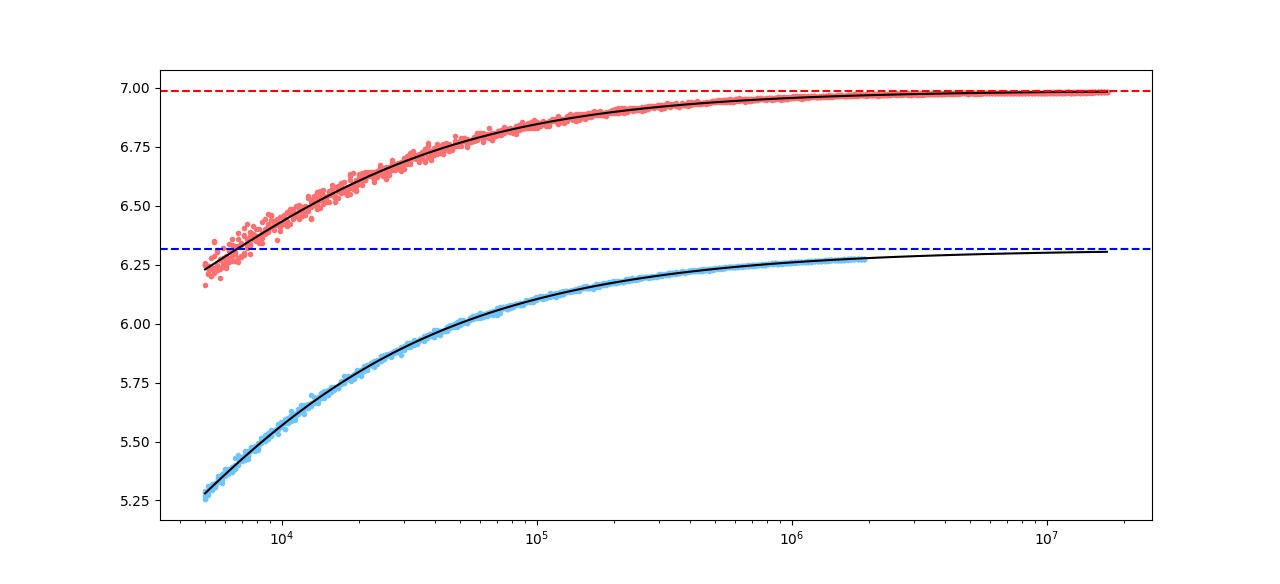
\includegraphics[width=\linewidth]{english_latin}
%\end{figure}

Although this method allows us to extrapolate from a small corpus, there's still a risk that the corpus may not be representative. To test this, we used ``author jackknifing'': we gathered a list of the 14 authors who contributed at least 100,000 tokens to the corpus, then performed the calculation repeatedly, removing a different one of these authors each time. The standard deviation of the results gives an approximation of how much the entropy value could be swayed by any particular author's style.

\section{Results and Discussion}

With these methods, we estimated a conditional entropy of 6.32 bits per syllable, with a standard error of 0.033. Combining this with Coupé's proposed universal information rate, we were able to determine the rate at which Classical Latin would have been spoken by native speakers thousands of years ago: 6.19 syllables per second, with a standard deviation of 0.81. While the variance is relatively large, it's almost entirely due to differences in speech rate within a language, with the uncertainty in our extrapolation being negligible.

Notably, our results indicate that Classical Latin was spoken at a significantly slower rate than modern Romance languages---Coupé's data shows a mean value of 7.73 syl/sec for Spanish, for example, and 7.16 syl/sec for Italian. This makes sense from a diachronic perspective, as historical sound changes generally reduced the size of the syllable inventory, decreasing the amount of information provided by each syllable.

This suggests multiple avenues for further research. These methods could be applied directly to other languages for which only written corpora exist; the primary difficulty lies in automatically creating phonemic representations from ambiguous writing systems, as it's unclear how well Winge's methods can be generalized. With Latin in particular, it should also be possible now to calculate the effects of the various sound changes that led to modern Romance languages, and determine how much the speech rate was affected by vowel shifts, epenthesis, coda deletion, and so on. Putting these changes into their historical context, this would allow us to predict speech rate across time and see when and why it changed over the centuries.

\nocite{*}

\printbibliography

\end{document}
